% ATTIVAZIONE NOTE (notes=show/only/none)
\documentclass[notes=show]{beamer}
%\documentclass{beamer}

\usetheme{Sapienza}

\usepackage[italian]{babel}
\usepackage[T1]{fontenc}
\usepackage[utf8]{inputenc}
\usepackage{ae}
\usepackage{float}
\usepackage{color}
\usepackage{tabularx}
\usepackage{multirow}
\usepackage{multicol}

\usepackage{listings}


\definecolor{dkgreen}{rgb}{0,0.6,0}
\definecolor{gray}{rgb}{0.5,0.5,0.5}
\definecolor{mauve}{rgb}{0.58,0,0.82}

\lstset{frame=tb,
  language=Java,
  aboveskip=3mm,
  belowskip=3mm,
  showstringspaces=false,
  columns=flexible,
  basicstyle={\small\ttfamily},
  numbers=none,
  numberstyle=\tiny\color{gray},
  keywordstyle=\color{blue},
  commentstyle=\color{dkgreen},
  stringstyle=\color{mauve},
  breaklines=true,
  breakatwhitespace=true,
  tabsize=3
}

\newenvironment{red_list}
 {\begin{list}{\scriptsize{\textcolor{red}{$\diamond$ }}}{\leftmargin=1em \itemindent=0em}}
 {\end{list}}
\newenvironment{green_list}
 {\begin{list}{\scriptsize{\textcolor{dgreen}{$\diamond$ }}}{\leftmargin=1em \itemindent=0em \labelwidth=0.5em}}
 {\end{list}}

% COLORI
\definecolor{dgreen}{rgb}{0.,0.6,0.}
\definecolor{dgrey}{rgb}{0.664,0.664,0.664}

% Hide presentation controls
\usenavigationsymbolstemplate{} 

\graphicspath{ {./Images/} }

 


% FINE PREAMBOLO

\setbeamercolor{bgcolor}{fg=white,bg=rosso_Sapienza}
\defbeamertemplate*{title page}{customized}[1][]
{	\begin{center}
		
\includegraphics[height=1.60cm]{logo_sapienza}\\
		\usebeamerfont{institute}\insertinstitute
	\end{center}
	\bigskip
	\begin{beamercolorbox}[rounded=true, center, shadow=false, ht=6.5ex, wd=.8\paperwidth]{bgcolor}
		\usebeamerfont{title}\inserttitle\par%
	\end{beamercolorbox}
\hfill\null\\
\smallskip\smallskip
{Relatore:}\hfill {Candidato:}\\
\textbf{Prof. Irene Finocchi}\hfill \textbf{\insertauthor}\\
\bigskip\bigskip
}

\title{Sviluppo e sperimentazione di algoritmi su grafi in Pregel e Mapreduce\smallskip}
%\subtitle{}
\author{Luigi Piccioli}
%\date{\today}
\institute{\normalsize\rmfamily\scshape{Facoltà di Ingegneria dell'Informazione, Informatica e Statistica}}
%\date{}


\begin{document}

% COPERTINA
\frame {
	\titlepage

\note{\footnotesize{
Buongiorno, mi chiamo Luigi Piccioli e mi presento con la tesi dal titolo ``Sviluppo e sperimentazione di algoritmi su grafi in Pregel e Mapreduce''.

}
}
}

% INTRODUZIONE
\section{Introduzione}
\frame {
	
	\textbf{Obiettivo:}\\
	\smallskip
	Sviluppo e sperimentazione di algoritmi su grafi in Pregel e Mapreduce.

	\bigskip
	\textbf{Organizzazione della presentazione:}
	\smallskip
	\begin{itemize}
		\item Il Modello MapReduce.
		\smallskip
		\item Il Modello Pregel.
		\smallskip
		\item Algoritmi Sviluppati.
		\smallskip
		\item Risultati.
		\smallskip
		\item Conclusioni e sviluppi futuri.
	\end{itemize}

% NOTE
\note{\footnotesize{
L'obiettivo di questa tesi è per l'appunto quello di sviluppare una serie di algoritmi su grafi sia sul modello Pregel che sul modello MapReduce\\\smallskip\smallskip

La presentazione è suddivisa in cinque sezioni organizzate nel seguente modo: Le prime due parti dove introdurrò  questi due modelli.\\\smallskip\smallskip

Una terza parte in cui verranno introdotti gli algoritmi sviluppati e le implementazioni MapReduce e Pregel.\\\smallskip\smallskip

Una quarta parte in cui sono mostrati i risultati ottenuti dalle sperimentazioni effettuate su un cluster di macchine degli algoritmi realizzati.\\\smallskip\smallskip

Ed infine alcune conclusioni sui risultati ottenuti da questo lavoro.

}
}
}

\section{MapReduce}

\frame
{
	\frametitle{MapReduce}
	
	Modello per il calcolo parallelo e distribuito di grandi quantità di dati su cluster composto da:	\\\smallskip\smallskip
	
	\begin{itemize}
		\item Modello di Programmazione
			\begin{itemize}
				\item Map
				\item Reduce\\\smallskip\smallskip
			\end{itemize}
		\item Architettura
			\begin{itemize}
				\item Gestione delle risorse del cluster
				\item Controllo flusso del programma
				\item Controllo e recupero degli errori
			\end{itemize}			
	\end{itemize}
	
	

	\smallskip

% NOTE
\note{\footnotesize{

MapReduce è un modello per il calcolo parallelo e distribuito di grandi qunatità di dati su un cluster di computer.

Il modello definisce sia il modello di programmazione (basato dalle funzioni Map e Reduce) che l'architettura su cui è eseguito un programma MapReduce.

In questo modo sono mantenute separate ed indipendenti le componenti implementative dell’algoritmo dal framework che si occupa della Gestione delle risorse del cluster, del controllo dell’esecuzione del flusso del programma, del controllo degli errori e del recupero successivo al guasto di una o più macchine del cluster.

}
}
}

\frame
{
	\frametitle{MapReduce - Modello di Programmazione}

	Funzioni base:
	\begin{itemize}
		\item Map\
		\begin{equation}
		MAP (k_{in},v_{in}) \rightarrow   (k_{out}, list(v_{out}))
		\end{equation}
		\item Reduce
		\begin{equation}
		REDUCE (k_{in}, list(v_{in})) \rightarrow   list(v_{in})
		\end{equation}
	\end{itemize}
	\begin{figure}
		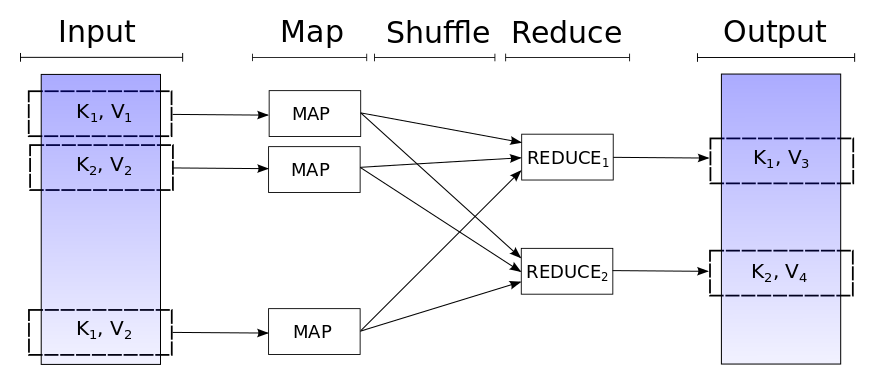
\includegraphics[width=0.8\textwidth]{MR_def_contesto}	
	\end{figure}
% NOTE
\note{\footnotesize{
Un programma MapReduce viene definito dalle funzioni base Map e Reduce.

Una programma MapReduce è composto da tre fasi principali:

\begin{itemize}
	\item Map
	\item Shuffle
	\item Reduce
\end{itemize}

Nella prima fase, l'input iniziale  viene suddiviso e inviato ad un processo che esegue la funzione Map. Questa funzione prende in input una coppia di chiave e valore e restituisce in output una lista di valori associati ad una chiave.

Nella seconda fase agisce, in modo traspare, la funzione Shuffle che raggruppa i valori in output delle funzioni di Map che condividono la stessa chiave.

Nella terza ed ultima fase viene eseguita la funzione Reduce la quale prende in input una chiave ed una lista di valori e restituisce una seria di valori in output.




}
}
}

\frame
{
	\frametitle{MapReduce - Architettura}
	
	\begin{figure}
		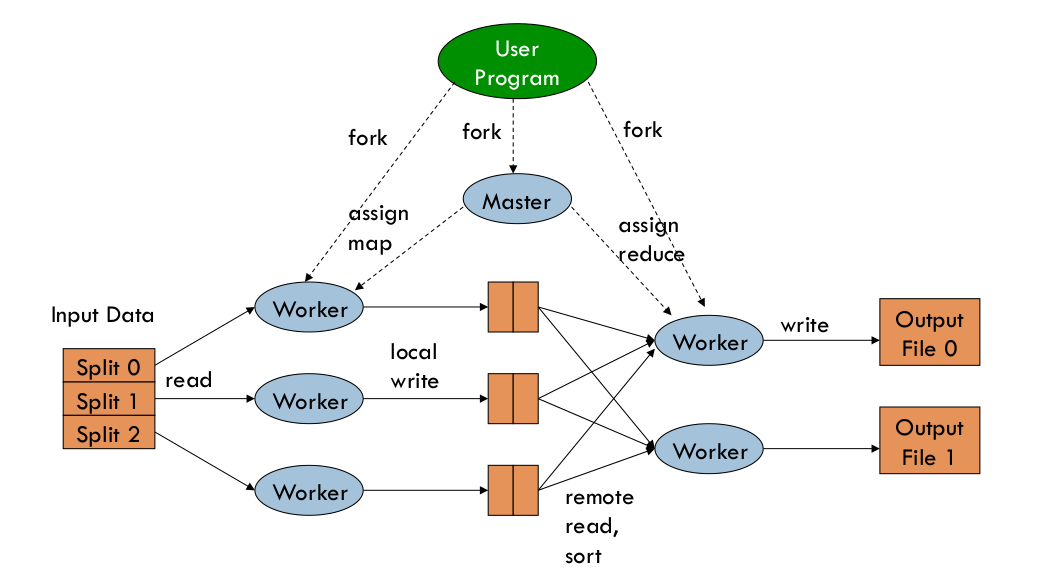
\includegraphics[width=\textwidth]{esempio_architettura}
		\caption{Architettura MapReduce }	
	\end{figure}
	
	
	
% NOTE
\note{\footnotesize{

L'architettura MapReduce è di tipo Master/Slave. E' composta da un nodo Master che si
occupa della gestione del flusso dei dati e dell'assegnazione dei task a tutti i nodi del
cluster chiamati Worker. 
Il Master assegna ai Worker di volta in volta le funzioni di MAP o le funzioni di REDUCE.

il flusso del programma  MapReduce si svolge nel seguente modo :

\begin{enumerate}
\item L'input del programma viene suddiviso in N parti distinte aventi la stessa dimensione tramite una funzione di partizione.

\item Le copie del programma vengono distribuite a tutte le macchine del cluster.

\item Il Master controlla quali worker sono disponibili ed assegna loro i task Map e Reduce da svolgere.

\item I Worker che ricevono un task MAP caricano i dati dall'input, leggono le coppie chiave valore e
 salvano nella memorie locali i risultati intermedi.
 
\item I risultati salvati localmente vengono ripartiti utilizzando la funzione di partizione.

\item Il nodo Master riceve la posizione dei risultati partizionati e la comunica ai Reducer a cui sono assegnate la
 partizioni.
 
\item I Reducer caricano i dati di una partizione dalle memorie locali dei Mappered eseguono la funzione REDUCE e producono in output i risultati.

\end{enumerate}
}
}
}

\frame
{
	\frametitle{MapReduce - Esempio}
	
	\textbf{Calcolo grado vertici del grafo}
	\begin{figure}
		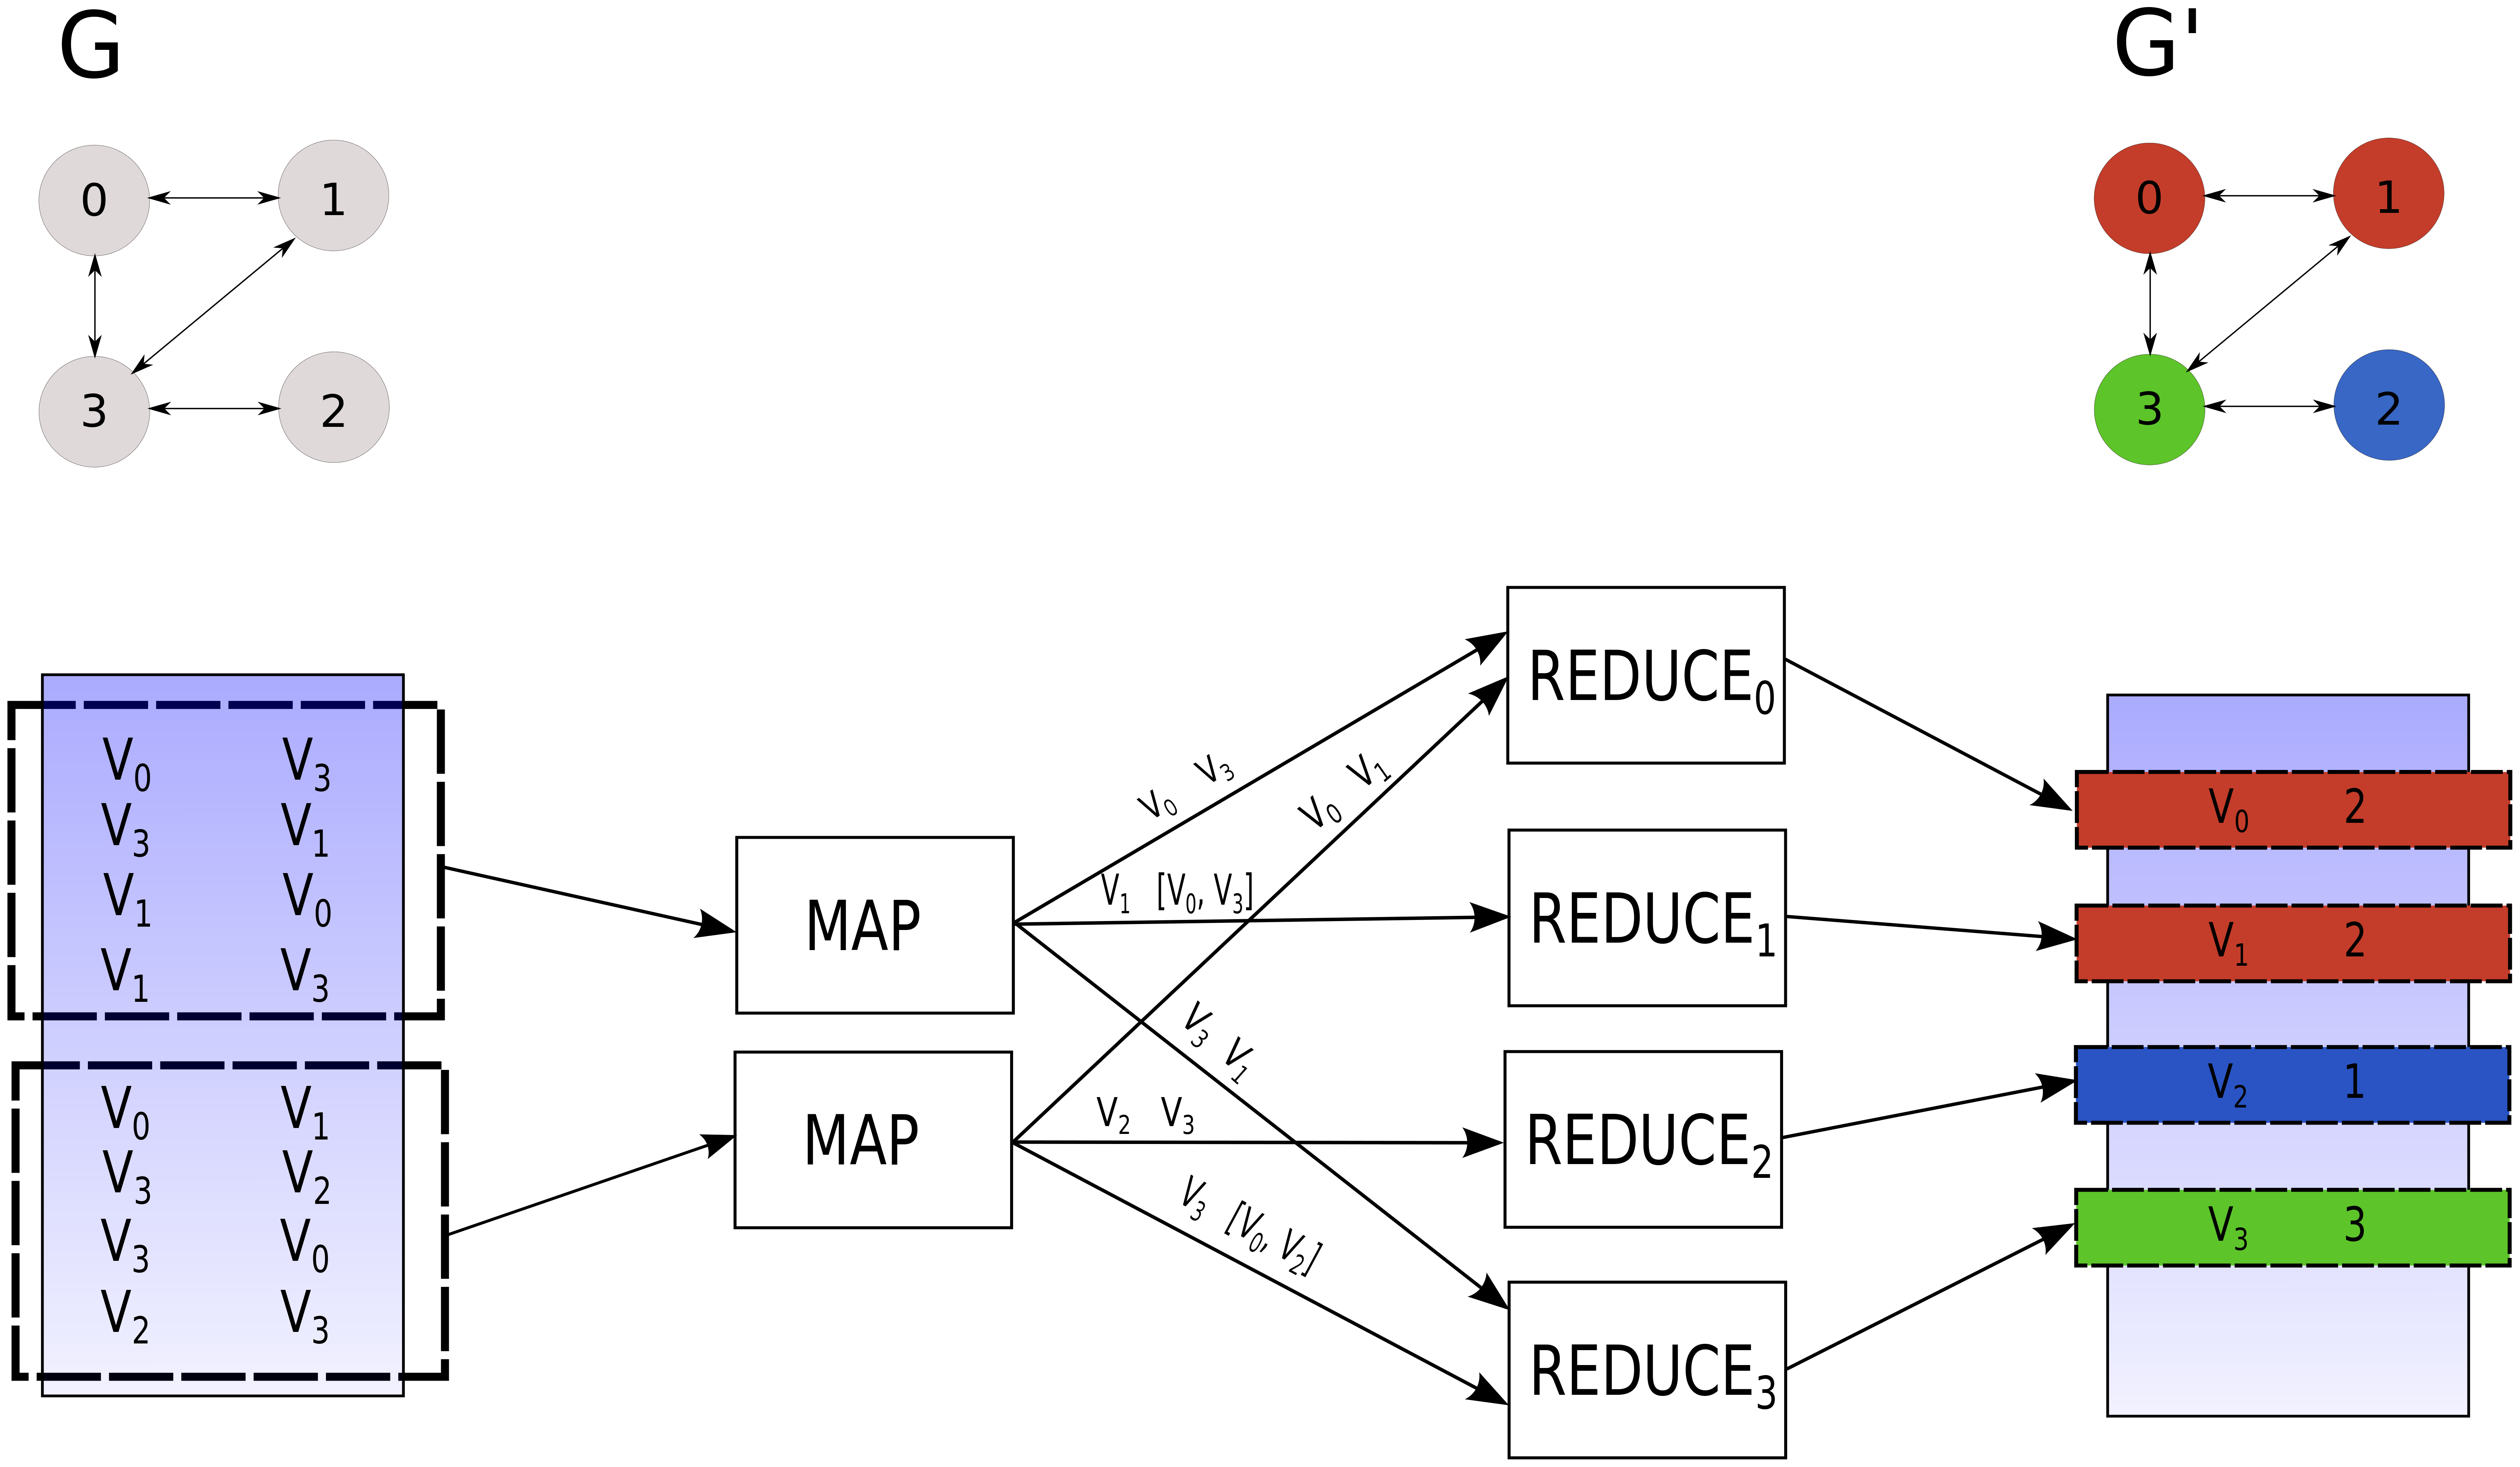
\includegraphics[width=\textwidth]{MR-DegreeCalculator}
		\caption{Esempio MapReduce - Grado dei vertici del grafo }	
	\end{figure}
	
	
% NOTE
\note{\footnotesize{

Un esempio di implementazione di un programma MapReduce su grafi e il calcolo del grado dei vertici che compongono il grafo.

L'input, formato di lista archi del grafo, viene suddiviso e associato ad un Mapper che restituisce per ogni nodo la lista dei vertici vicini.

Ogni reduce riceve  in input un nodo e la lista di tutti ad esso nodi adiacenti, li conta e restituisce in output il risultato che rappresenta il grado del vertice.

%TODO, riscrivere seguendo i passaggi di V3 -> MAP2 -> REDUCE3

}
}
}

\section{Pregel}

\frame
{
	\frametitle{Modello Pregel}
	
	Modello per il calcolo parallelo e distribuito di \textit{grafi} di grandi dimensioni su cluster composto da:	\\\smallskip\smallskip
	
	\begin{itemize}
		\item Modello di Programmazione
		\begin{itemize}
			\item Basato sul modello Bulk Synchronous Parallel (BSP)
			\item Vertice Centrico
			\\\smallskip\smallskip
		\end{itemize}
		\item Architettura
		\begin{itemize}
			\item Gestione delle risorse del cluster
			\item Controllo flusso del programma
			\item Controllo e recupero degli errori
		\end{itemize}
	\end{itemize}
	
	
% NOTE
\note{\tiny{
Pregel è un modello per l'esecuzione distribuita, parallela  di algoritmi su grafi su cluster di computer.

Pregel può essere definito come una specializzazione di MapReduce  sui grafi, infatti viene definito sia il modello di programmazione che l'architettura su cui andare ad eseguire un programma in Pregel.

Il modello di programmazione si definisce vertice centrico in quanto la logica dell'intero programma dipende dalla funzione base del modello che definisce le azioni che sarranno eseguite dai vertici del grafo durante le varie iterazioni.
}
}
}

\frame
{
	\frametitle{Pregel - Modello di Programmazione}
	
	\textbf{Basato sul modello Bulk Synchronous Parallel (BSP)} \\\smallskip
	
	Modello computazionale astratto per la progettazione di algoritmo
paralleli
	
	\begin{columns}[t]
	\begin{column}{0.5\textwidth}
	\begin{itemize}
			\item \textbf{Calcolo concorrente}\smallskip
			\item \textbf{Comunicazione}\smallskip
			\item \textbf{Barriera di sincronizzazione}\smallskip
		\end{itemize}
	\end{column}
	\begin{column}{0.5\textwidth}\\\smallskip
		\vspace{-3em}
		\begin{figure}
			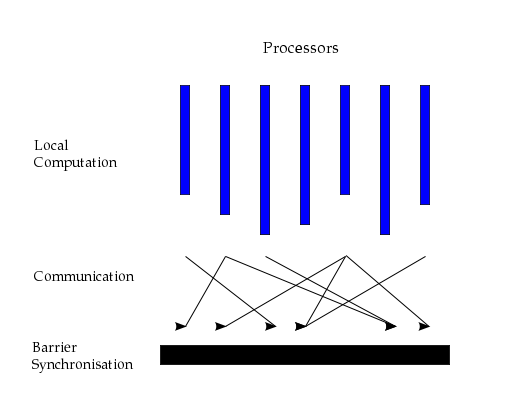
\includegraphics[width=\textwidth]{BSP}
			\caption{BSP}	
		\end{figure}
		\end{column}
	\end{columns}
	

% NOTE
\note{\scriptsize{
Il modello \textit{Pregel} si basa sul  il\textbf{ Bulk Synchronous Parallel (BSP) Model} che  è un modello computazionale astratto per la progettazione di algoritmo paralleli.

Una macchina è costituita da più processori, ognuno avente la propria memoria locale indipendente e connessi tra loro da una rete di comunicazione.

Una computazione in questo modello è composta da una serie di superstep globali, in ogni superstep:
\begin{itemize}
\item \textbf{Calcolo concorrente}: un prima fase in cui ogni processore che partecipa al superstep effettua le operazioni utilizzando la propria memoria locale.
\item \textbf{Comunicazione}: nella fase di comunicazione i processori scambiano dati tra loro.
\item \textbf{Barriera di sincronizzazione}: Quando un processo che raggiunge questo step rimane in stato di attesa fino a quando tutti i processi non hanno terminato la fase precedente.
\end{itemize}
}
}
}

\frame
{

	\frametitle{Pregel - Modello di Programmazione}
	
	\begin{itemize}
		\item Modello \textbf{vertice-centrico}
		\item Computazione divisa in \textit{superstep}
	\end{itemize}
	
	\begin{columns}[t]
	\begin{column}{0.6\textwidth}
		
	\smallskip\smallskip
	
	Ad ogni superstep \textit{S} il vertice \textit{V}:
	\begin{enumerate}
		\item Riceve messaggi inviati al superstep \textit{S-1}.
		\item Altera lo stato del Vertice \textit{V}.
		\item Invia messaggi che verranno ricevuti al superstep \textit{S+1}.
	\end{enumerate}
	\end{column}
	\begin{column}{0.4\textwidth}\\\smallskip
		\begin{figure}
			\includegraphics[width=\textwidth]{Pregel_stati}
			\caption{Diagramma stati vertice in Pregel}	
		\end{figure}
	\end{column}
	\end{columns}

% NOTE
\note{\scriptsize{
La computazione di un programma definito secondo il modello \textbf{Pregel} è suddivisa in superstep. 

Ad ogni \textit{superstep} viene eseguita la funzione base del modello che prevede la ricezione dei messaggi inviati nell'iterazione precedente, la modifica dello stato del vertice e l'invio di messaggi ai vertici che li riceveranno nel superstep successivo. 

Nella figura mostrata sulla slide è rappresentato il diagramma degli stati che un vertice può raggiungere durante l'esecuzione del programma in Pregel.
All'inizio dell'esecuzione tutti i vertici si trovano in uno stato Active, nel corso di ogni superstep un vertice può decidere di passare ad uno stato Vote to Halt. Un vertice non esegue alcuna azione quando si trova in questo stato, fintantoché non rieve un messaggio in entrata da un altro vertice, in questo caso torna ad uno stato Active  nel corso dello stesso Superstep. 

L'esecuzione del programma termina quando tutti i vertici si trovano in uno stato Vote to halt.
}
}
}

\frame
{

	\frametitle{Pregel - Esempio SSSP }
	
	Cammini minimi da sorgente singola
	\begin{columns}[t]
	\begin{column}{0.6\textwidth}
	\begin{figure}
			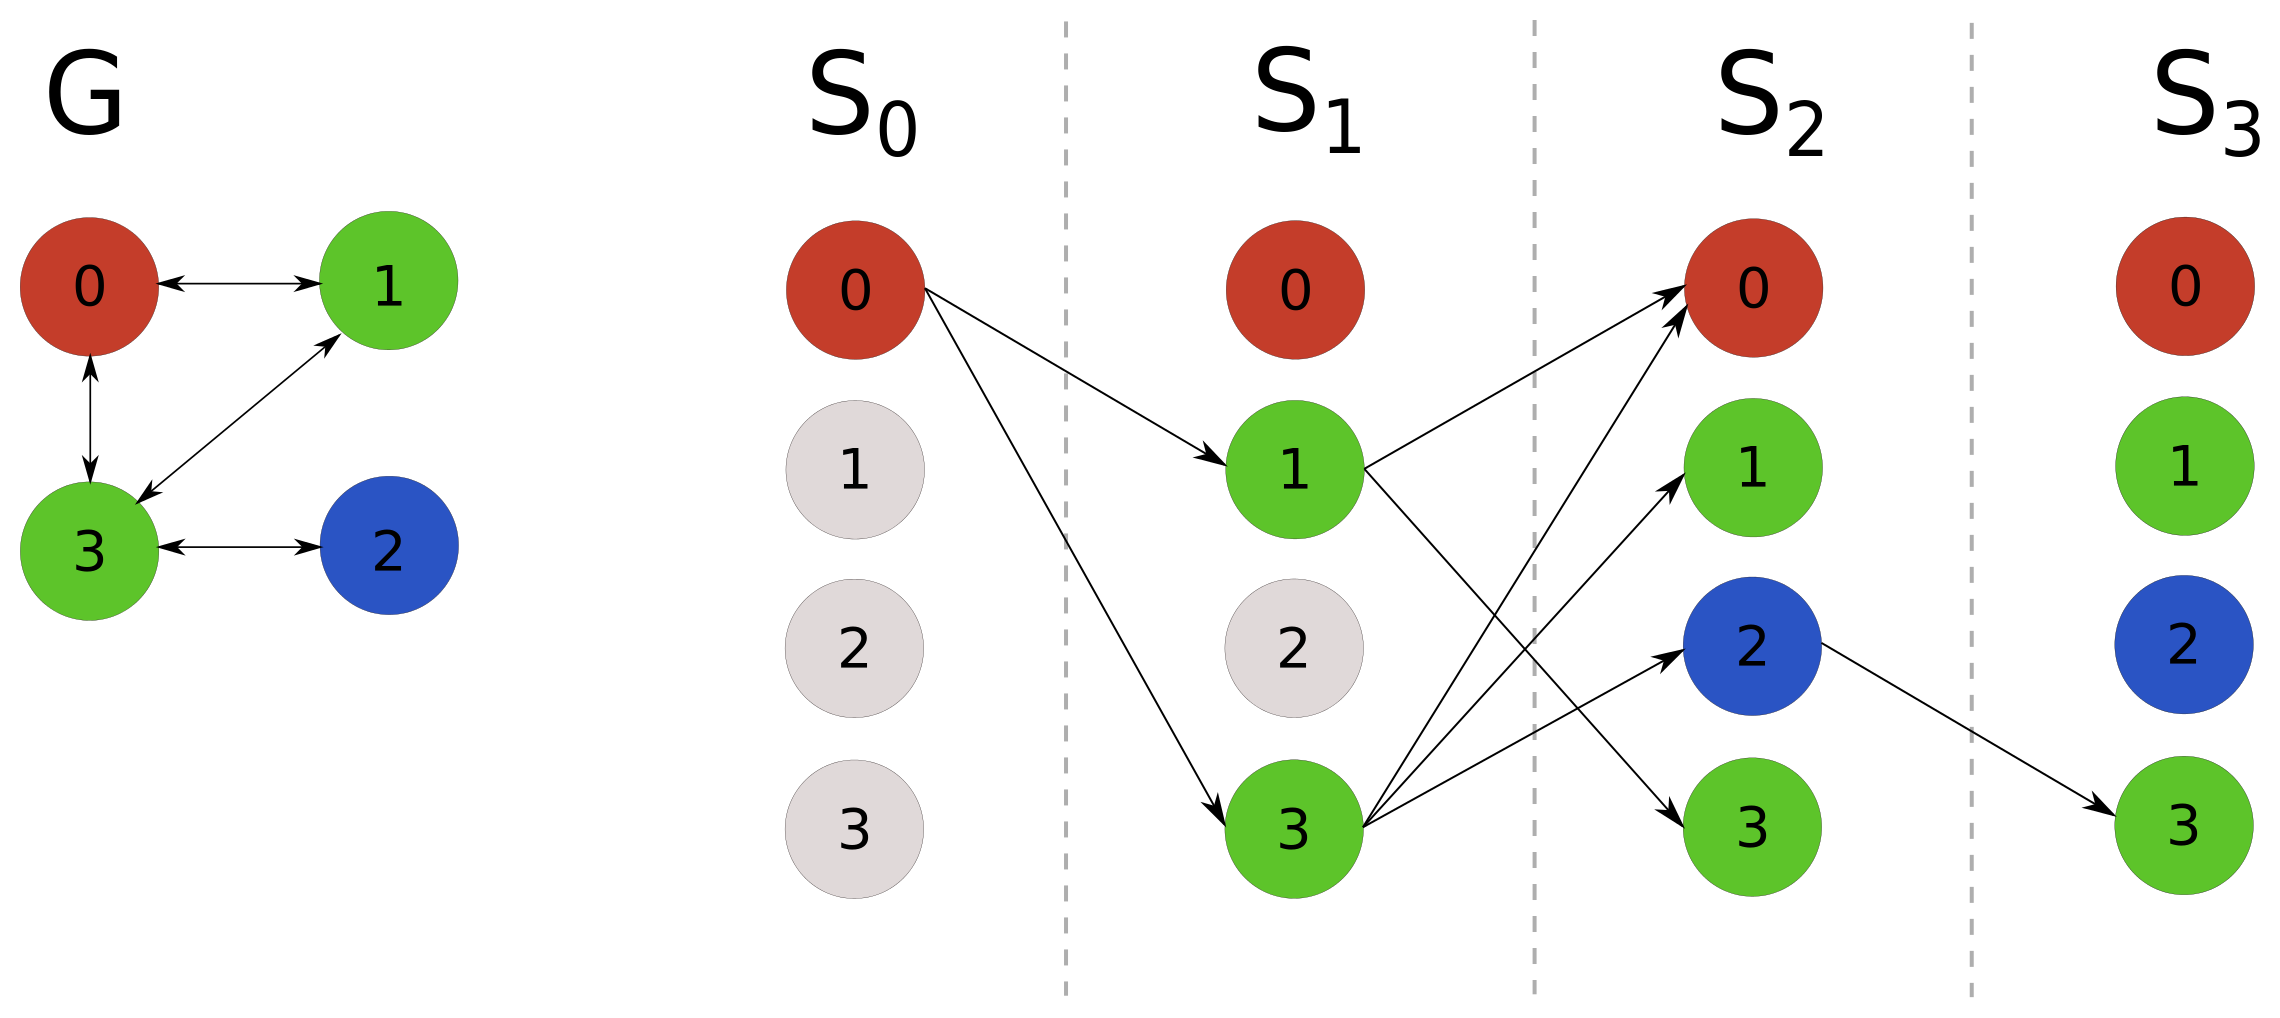
\includegraphics[width=\textwidth]{PREGEL-SSSP}
			\caption{Pregel - Esempio SSSP}	
	\end{figure}
	\end{column}
	\begin{column}{0.4\textwidth}
	
		TODO:INSERIRE PSEUDOCODICE
	
	\end{column}
	\end{columns}
	


% NOTE
\note{\scriptsize{

	

}
}
}

\frame
{

	\frametitle{Pregel - Architettura}
	
	\begin{figure}
			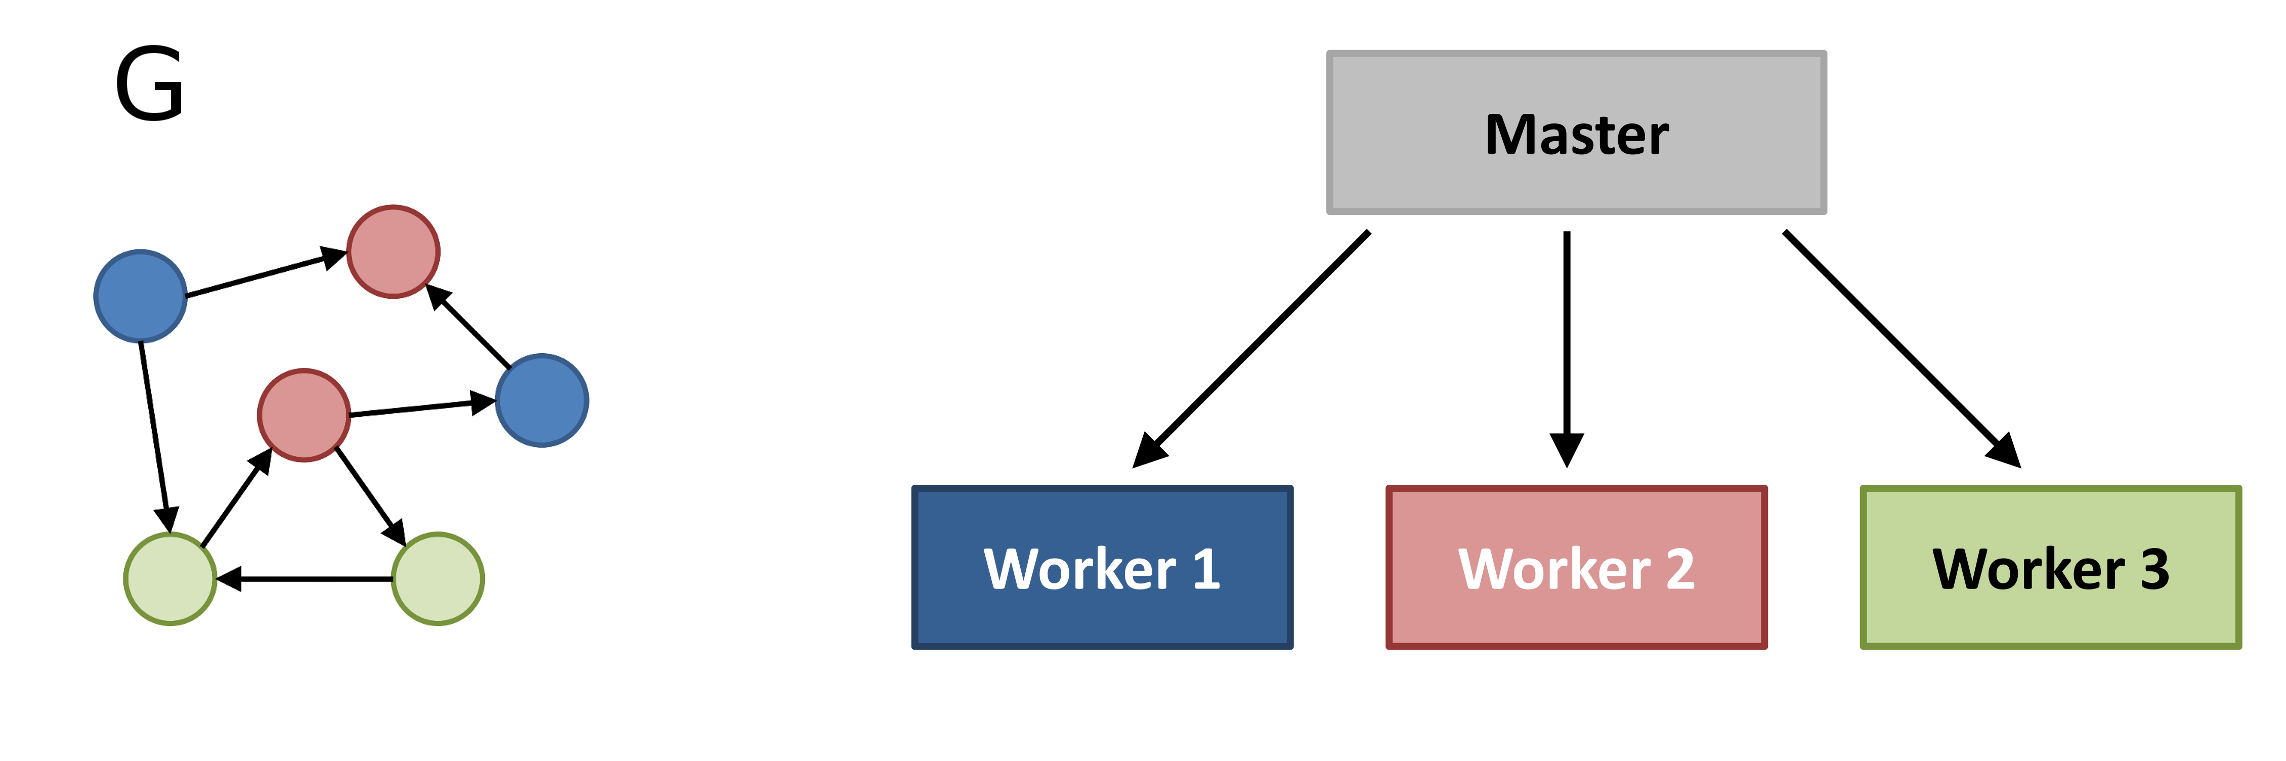
\includegraphics[width=\textwidth]{partizionePregel}
			\caption{Architettura Pregel}	
	\end{figure}
	

% NOTE
\note{\scriptsize{

}
}
}


%
%\frame
%{
%	\frametitle{Berlin A5/1 rainbow table set}
%	
%	Costituiscono il cuore dell'attacco al cifrario A5/1.\\
%	\smallskip\smallskip\smallskip
%	L'idea è quella di creare un insieme di tabelle che associa (``mappa'') ogni possibile sequenza di 64 bit che compone lo stato interno dei registri LFSR ai primi 64 bit della \textit{keystream} da essi prodotta.\\
%
%	\smallskip\smallskip\smallskip
%
%	Conoscendo il \textit{frame number} e lo stato interno dei registri è possibile effettuare il \textit{back-clock} dei tre LFSR e risalire alla chiave di sessione $K\ped{c}$ utilizzata.\\
%
%%	\begin{center}
%%		\includegraphics[width=\textwidth]{ricerca_e_back_clock}
%%	\end{center}
%
%\bigskip
%
%
%% NOTE
%\note{\footnotesize{
%
%Il dizionario utilizzato per questa tesi prende il nome di ``Berlin A5/1 rainbow table set'' o più semplicemente ``Berlin tables'' e consiste in un insieme di tabelle che sfruttano il concetto del time-memory trade-off per associare ogni possibile sequenza di 64 bit che compone lo stato interno dei registri ai primi 64 bit della keystream da essi prodotta.\\\smallskip\smallskip 
%
%Ottenuto lo stato interno dei registri e conoscendo il frame number del messaggio, che è un parametro noto, è quindi possibile eseguire quello che viene chiamato ``back-clock'' dei registri e risalire quindi alla chiave di sessione K\ped{c} inserita durante la fase di inizializzazione e utilizzata per generare tutte le keystream.
%
%}
%}
%}
%
%\frame
%{
%	\frametitle{Berlin A5/1 rainbow table set}
%
%	Si presentano al download come un insieme di 40 tabelle:\smallskip
%		
%	\begin{itemize}
%		\item Ognuna ha una dimensione di 42 GB.\smallskip\smallskip\smallskip
%		\item La dimensione totale è di circa 1.7 TB.\smallskip\smallskip\smallskip
%		\item La copertura stimata è pari a circa il 19\% dello spazio\\\smallskip totale degli stati, ovvero $2^{61}$ possibili chiavi.\smallskip\smallskip\smallskip
%		\begin{itemize}
%		\item Dimezzare il numero di chiavi implica raddoppiare il numero delle catene calcolate.
%			\end{itemize}\smallskip\smallskip\smallskip
%		\item Per essere utilizzate necessitano di un processo preliminare di indicizzazione.\smallskip\smallskip\smallskip
%		\item Ogni tabella è identificata da un ID univoco:
%	\end{itemize}
%
%	\begin{table}[H]
%	        \centering\scriptsize
%	        \begin{tabular}{|c|c|c|c|c|c|c|c|c|c|}\hline
%		        100&108&116&124&132&140&148&156&164&172\\ \hline
%		        180&188&196&204&212&220&230&238&250&260\\ \hline
%		        268&276&284&292&324&332&340&348&356&364\\ \hline
%		        372&380&388&396&404&412&420&428&492&500\\ \hline
%	        \end{tabular}
%	\end{table}
%	
%% NOTE
%\note{\footnotesize{
%Le ``Berlin tables'', nella versione attuale, si presentano al download come un insieme di 40 tabelle ognuna di dimensione 42 Gigabyte per un totale di circa 1.7 Terabyte. Nonostante le dimensioni particolarmente generose, la copertura stimata è pari a circa il 19\% dello spazio totale degli stati, ovvero $2^{61}$ possibili chiavi.\\\smallskip\smallskip
%
%Aumentare la copertura è possibile costruendo altre tabelle, ma con la tecnica attuale è stimato che per dimezzare il numero di chiavi assenti sarebbe necessario raddoppiare il numero delle catene calcolate, con importanti conseguenze sull'occupazione di memoria.\\\smallskip\smallskip
%
%Vista la dimensione di queste tabelle, il loro utilizzo prevede una fase preliminare di indicizzazione e questo, assieme la ricerca all'interno di esse è possibile per mezzo di una suite di programmi dedicati che prende il nome di Kraken.
%
%}
%}
%}
%
%
%%\section{Kraken}
%
%\frame
%{
%	\frametitle{Kraken}
%	Fornisce gli strumenti per utilizzare le \textit{Berlin tables} ed eseguire l'attacco al cifrario A5/1.
%	
%	\smallskip\smallskip\smallskip
%	
%	Permette di:
%
%	\vskip-1em
%	\begin{columns}[t]
%	\begin{column}{0.56\textwidth}
%		\smallskip\begin{itemize}
%		\item Indicizzare le \textit{Berlin tables}.\smallskip\smallskip
%		\item Eseguire l'operazione di XOR tra stringhe binarie.\smallskip\smallskip
%		\item Eseguire la ricerca di una \textit{keystream} all'interno delle \textit{Berlin tables}.\smallskip\smallskip
%		\item Eseguire l'operazione di \textit{back-clock} dei registri e ricavare la chiave di sessione $K\ped{c}$.
%		\end{itemize}	
%	\end{column}
%%	\begin{column}{0.48\textwidth}\\\smallskip
%%		\vspace{-3.2em}\includegraphics[width=\columnwidth]{suite_kraken_slides}
%%	\end{column}
%	\end{columns}
%
%% NOTE
%\note{\footnotesize{
%
%Kraken è appunto una suite e fornisce tutti gli strumenti necessari per utilizzare le tabelle e completare l'attacco al cifrario A5/1. Grazie ad essa è infatti possibile indicizzare le tabelle per prepararle al loro utilizzo, eseguire la ricerca di una keystream all'interno di esse e, in caso di successo, eseguire anche l'operazione di back-clock dei registri e calcolare quindi la chiave di sessione K\ped{c} utilizzata per la cifratura.
%
%}
%}
%}


\section{Algortimi su grafi}
% TEST
\section{Test}

% CONCLUSIONI
\section{Conclusioni}

% COPERTINA
\section*{}
\begin{frame}%[noframenumbering]
	\titlepage

	% NOTE
	\note{\footnotesize{Grazie :)}}
\end{frame}


\end{document}
